\section{Bayesian Coresets}
\label{sec:bayesian-coresets}

In this work, the goal is to approximate expectations under a density $\pi(\theta)$, 
 \mbox{$ \theta \in \Theta $} expressed as the product of $N$ potentials 
$ (f(x_n, \theta))_{n=1}^{N} $ and a base density $ \pi_0(\theta)$:
\[
\pi(\theta) &\defined \frac{1}{Z} \exp \left(\sum_{n=1}^{N} f(x_n, \theta)\right) \pi_0(\theta).\label{eq:posterior}
\]
In the setting of Bayesian inference with conditionally independent data, 
the potentials are data log-likelihoods, i.e. $f(x_n, \theta) := \log p(x_n | \theta)$,
 $\pi_0$ is the prior density, $\pi$ is the posterior, 
and $Z$ is the marginal likelihood of the data. 
Rather than working directly with $\pi(\theta)$ for 
posterior inference---which requires a $\Theta(N)$ computation per evaluation---a
Bayesian coreset approximation of the form
\[
\pi_w(\theta) \defined \frac{1}{Z(w)} \exp\left(\sum_{n=1}^N w_n f(x_n, \theta)\right)\pi_0(\theta)
\]
for $w\in\reals^N$, $w\geq 0$ may be used in most popular posterior inference schemes \citep{neal11,kucukelbir17,ranganath14}.
If the number of nonzero entries $\|w\|_0$ of $w$ is small, this results in a significant reduction in computational burden.
Recent work has formulated the problem of constructing a  Bayesian coreset of size $M\in\nats$ as sparse variational inference~\citep{campbell19neurips},
\[
& w^\star = \argmin_{w\in\reals^N} \kl{\pi_w}{\pi_1}\label{eq:coresets-vi} \quad \quad
 \text{s.t.} \quad w \geq 0, \; \|w\|_0 \leq M,
\]
and showed that the objective can be minimized using stochastic estimates of $\nabla_w\kl{\pi_w}{\pi_1}$
based on samples from the coreset posterior $\pi_w$. 

\subsection{High-dimensional data}
\label{sec:high_dimensional_data}


Coresets, as formulated in~\cref{eq:coresets-vi}, are limited to using the
original datapoints themselves to summarize the whole dataset.
\cref{prop:original_coreset_fails} shows that this is problematic when
summarizing high-dimensional data; in the common setting of posterior inference
for a Gaussian mean, the KL divergence $\kl{\pi_{w^\star}}{\pi_1}$ of the
\emph{optimal} coreset of any size scales with the dimension of the data.  The
proof may be found in~\cref{supp:proofs}.
\bnprop \label{prop:original_coreset_fails}
Suppose we use $(X_n)_{n=1}^N \distiid \distNorm(0, I)$ in $\reals^d$ to perform posterior inference in a Bayesian model
with prior 
$\mu \dist \distNorm(0, I)$ and likelihood
$(X_n)_{n=1}^N  \distiid \distNorm(\mu, I).$
Then $\forall M < d$ and $\delta \in[0, 1]$, 
with probability at least $1-\delta$ the optimal size-$M$ coreset $w^\star$ satisfies
\[
\kl{\pi_{w^\star}}{\pi_1} \geq \frac{1}{2}\frac{N-M}{1+N}F_{d-M}^{-1}\left(\delta{N\choose M}^{-1}\right),
\]
where $F_{k}$ is the CDF of a $\chi^2$ random variable with $k$ degrees of freedom.
\enprop

In the setting of~\cref{prop:original_coreset_fails}, both the exact posterior and the coreset posterior 
are multivariate Gaussian distributions, denoted as $\distNorm{\left(\mu_1, \Sigma_1\right)}$ and 
$\distNorm{\left(\mu_{w}, \Sigma_{w}\right)}$ respectively. 
The mean and covariance are
\[
\Sigma_{1}=\frac{1}{1+ N} I_d, \quad \mu_{1}=\Sigma_{1}\left( \sum_{n=1}^{N} X_{n}\right), 
\label{eq:exact_post}
\]
and
\[
\label{eq:coreset_post}
\hspace{-.3cm}\Sigma_{w}\!=\!\frac{I_d}{1+ \left(\sum_{n=1}^N w_n\right)}, 
\quad
\mu_{w}\!=\!\Sigma_{w}\left( \sum_{n=1}^{N} w_n X_{n}\right).
\]

\begin{proof}[Proof of~\cref{prop:original_coreset_fails}]
	By~\cref{eq:exact_post,eq:coreset_post}, 
	\begin{equation} \label{eq:KL_from_coreset_post_to_exact}
	\begin{aligned}
	\kl{\pi_{w}}{\pi_1}
	=& \frac{1}{2}\left[\log\frac{|\Sigma_{1}|}{|\Sigma_{w}|} - d + \tr\left( \Sigma_{1}^{-1}\Sigma_{w}\right)   
	(\mu_{1} - \mu_{w})^T \Sigma_{1}^{-1}(\mu_{1} - \mu_{w})\right]\\
	=& \frac{1}{2} \left[ -d\log \left( \frac{1+ N}{1+ \sum_{n=1}^N w_n}\right) - d  + d \left( \frac{1+ N}{1+ \sum_{n=1}^N w_n}\right)
	+  (\mu_{1} - \mu_{w})^T \Sigma_{1}^{-1}(\mu_{1} - \mu_{w})\right].
	\end{aligned}
	\end{equation}
	Note that $\forall x > 0, x-1 \geq \log x$, implying that 
	$$ d\log \left( \frac{1+ N}{1+ \sum_{n=1}^N w_n}\right) -d + d \left( \frac{1+ N}{1+ \sum_{n=1}^N w_n}\right) > 0.$$ 
	Thus, 
	\begin{equation} \label{eq:first_inequality}
	\kl{\pi_{w}}{\pi_1} \geq \frac{1}{2}(\mu_{1} - \mu_{w})^T \Sigma_{1}^{-1}(\mu_{1} - \mu_{w}).
	\end{equation}
	
	Suppose we pick a set $\mcI\subseteq[N]$, $\left|\mcI\right| = M$ of active indices $n$ where the optimal $w_n \geq 0$,
	and enforce that all others $n\notin \mcI$ satisfy $w_n = 0$.
	Then denoting
	\[
	Y = \left[X_n : n\notin \mcI\right] \in \reals^{d\times (N-M)}, \quad
	X = \left[X_n : n\in \mcI\right] \in \reals^{d\times M},
	\]
	we have that for any $w\in \reals_+^M$ for those indices $\mcI$,
	\[
	\kl{\pi_w}{\pi_1} 
	\geq & \frac{1}{2(N+1)}1^TY^TY1 
	+1^TY^TX\left(\frac{1}{N+1} - \frac{w}{1+1^Tw}\right)\\
	&+\frac{N+1}{2}\!\!\left(\frac{1}{N+1}\! -\! \frac{w}{1+1^Tw}\right)^T\!\!\!\!\!X^T\!X\!\left(\frac{1}{N+1} \!-\! \frac{w}{1+1^Tw}\right).
	\]
	Relaxing the nonnegativity constraint, replacing $w/(1+1^Tw)$ with a generic $x\in\reals^M$, and 
	noting that $X^TX$ is invertible almost surely when $M < d$,
	we can optimize this expression yielding a lower bound
	on the optimal KL divergence using active index set $\mcI$,
	\[
	\kl{\pi_{w^\star_{\mcI}}}{\pi_1} &\geq \frac{1^TY^T\left(I-X(X^TX)^{-1}X^T\right)Y1}{2(N+1)}.
	\]
	The numerator is the squared norm of $Y1$ minus its projection onto the subspace spanned by the $M$ columns of $X$.
	Since $Y1 \dist \distNorm(0, (N-M)I)$, $Y1 \in \reals^d$ is an isotropic Gaussian, then its projection into the orthogonal
	complement of any fixed subspace of dimension $M$ is also an isotropic Gaussian of dimension $d-M$ with the same variance.
	Since the columns of $X$ are also independent and isotropic, its column subspace is uniformly distributed.
	So therefore, for each possible choice of $\mcI$
	\[
	\kl{\pi_{w^\star_{\mcI}}}{\pi_1} &\geq \frac{N-M}{2(N+1)} Z_{\mcI},  \quad Z_{\mcI}\dist \chi^2(d-M).
	\]
	Note that the $Z_\mcI$ will have dependence across the $N\choose M$ different choices of index subset $\mcI$.
	Thus, the probability that \emph{all} $Z_{\mcI}$ are large is
	\[
	\Pr\left(\min_{\mcI \subseteq [N], |\mcI| = M} Z_{\mcI} > \epsilon\right) 
	\geq &1 - {N\choose M}\Pr\left(Z_{\mcI} \leq \epsilon\right)\\
	= &1 - {N\choose M}F_{d-M}(\epsilon),
	\]
	where $F_{k}$ is the CDF for the $\chi^2$ distribution with $k$ degrees of freedom.
	The result follows.
\end{proof}

The bound in \cref{prop:original_coreset_fails} depends on $d$ through the
$\chi^2$ distribution inverse CDF. Although difficult to see directly, the
bound is reasonably large for typical values of $N, M, d, \delta$, and
increasing linearly in $d$; \cref{fig:klbound} visualizes the value of the
lower bound as a function of dimension $d$ for various coreset sizes $M$. Note
that the above bound requires the data to be high-dimensional such that $d >
M$; if $d\leq M$ the proof technique used above results in a vacuous
$\kl{\pi_{w^\star}}{\pi_1} = 0$ lower bound. 

\captionsetup[subfigure]{labelformat=empty}
\begin{figure}[t!]
	\centering 
\begin{subfigure}[b]{.47\textwidth} 
	\scalebox{1}{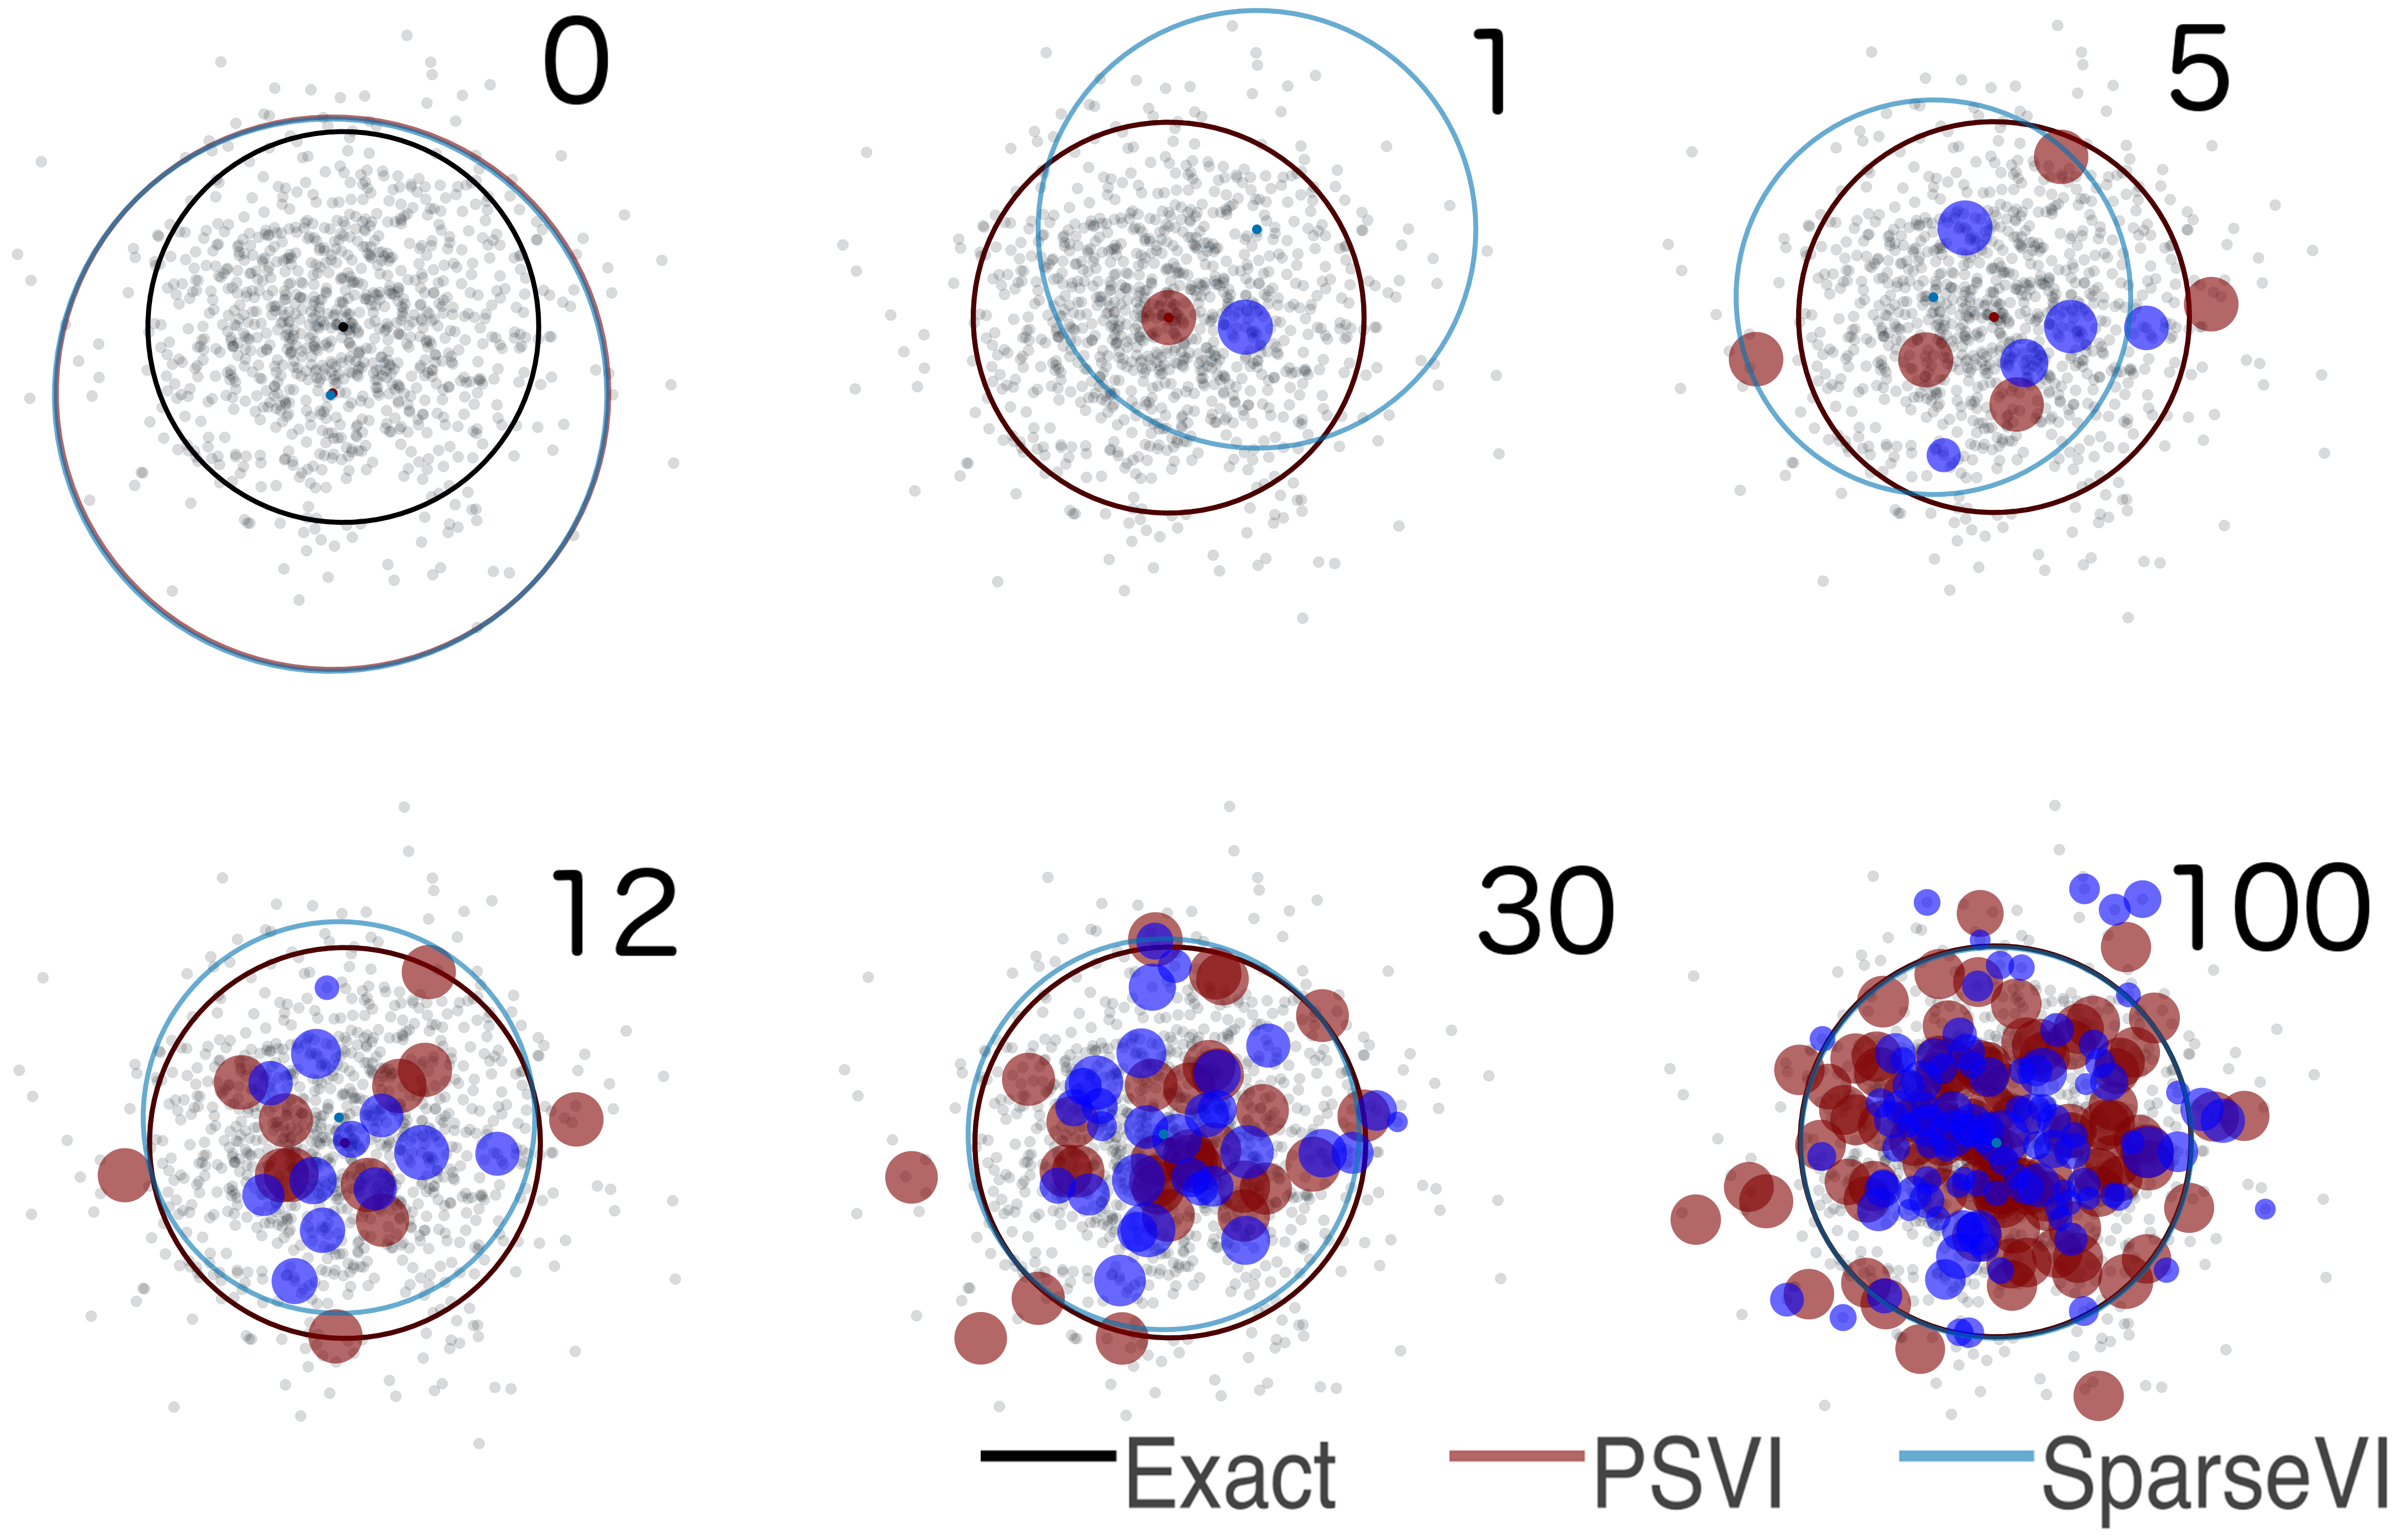
\includegraphics[width=\textwidth]{\MyPath/figs/d500_pts_combined.png}}
	\caption{(a)\label{fig:gaussian_coreset_points}}
	\end{subfigure}
\hfill\qquad
\centering
\begin{subfigure}[b]{0.47\textwidth}
	\scalebox{1}{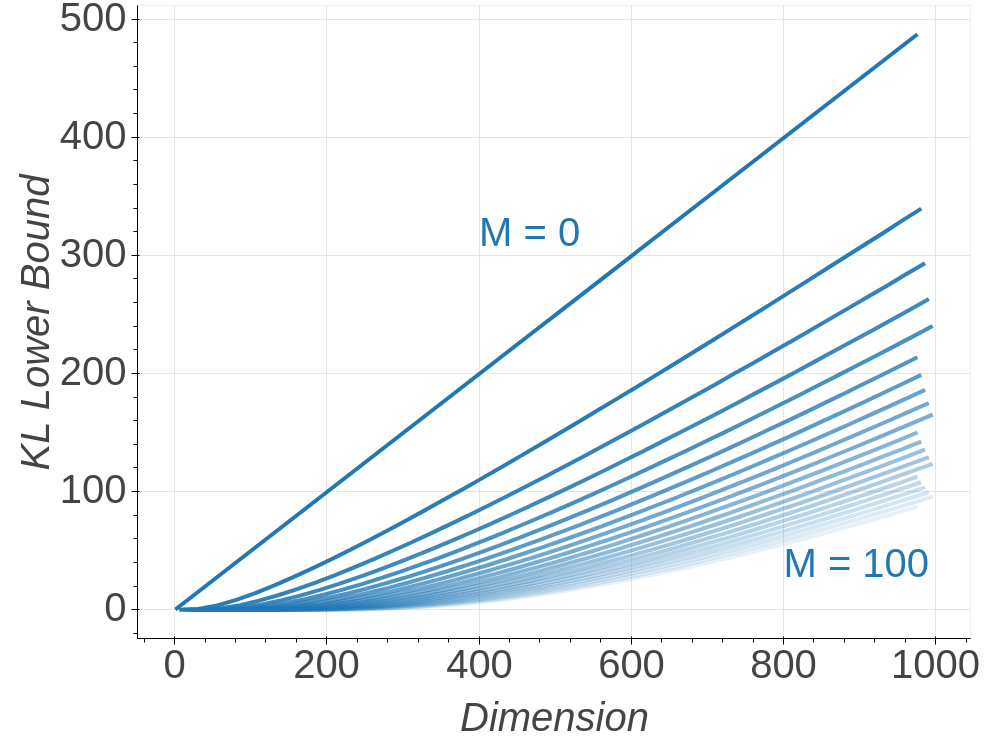
\includegraphics[width=\textwidth]{\MyPath/figs/klbound.png}}
	\caption{(b)\label{fig:klbound}}
\end{subfigure}
\caption{Gaussian mean inference under~pseudocoreset (\psvi)~against~standard coreset (\sparsevi) summarization for $N=1,000$  datapoints. (\subref{fig:gaussian_coreset_points})~Progression of~\psvi~vs.~\sparsevi~construction for coreset sizes $M=0, 1, 5, 12, 30, 100$, in 500 dimensions~(displayed are datapoint projections on 2 random dimensions).~\psvi~and~\sparsevi~coreset predictive $3\sigma$ ellipses are displayed in red and blue respectively, while the true posterior $3\sigma$ ellipse is shown in black.~\psvi~has the ability to immediately move pseudopoints towards the  true posterior mean, while \sparsevi~has to add a larger number of existing points in order to obtain a good posterior approximation. See \cref{fig:gaussian_dkl} for the quantitative KL comparison.
(\subref{fig:klbound})~Optimal coreset KL divergence lower bound from \cref{prop:original_coreset_fails} as a function of dimension with $\delta = 0.5$, and  coreset size $M$ evenly spaced from 0 to 100 in increments of 5.}
\end{figure}

